% Figure 5.5: Sequential (LSTM) Architecture
% Compile with: pdflatex fig_5_5_lstm_architecture.tex

\documentclass[border=10pt]{standalone}
\usepackage{tikz}
\usetikzlibrary{shapes.geometric, arrows.meta, positioning}
\usepackage{xcolor}
\usepackage{amsmath}

% Professional academic color palette
\definecolor{inputgray}{RGB}{220, 220, 220}
\definecolor{embedblue}{RGB}{176, 196, 222}    % Light steel blue
\definecolor{lstmteal}{RGB}{119, 176, 166}     % Muted teal
\definecolor{denseorange}{RGB}{222, 184, 135}  % Burlywood
\definecolor{outputpurple}{RGB}{186, 175, 201} % Lavender gray
\definecolor{textdark}{RGB}{33, 33, 33}

\begin{document}
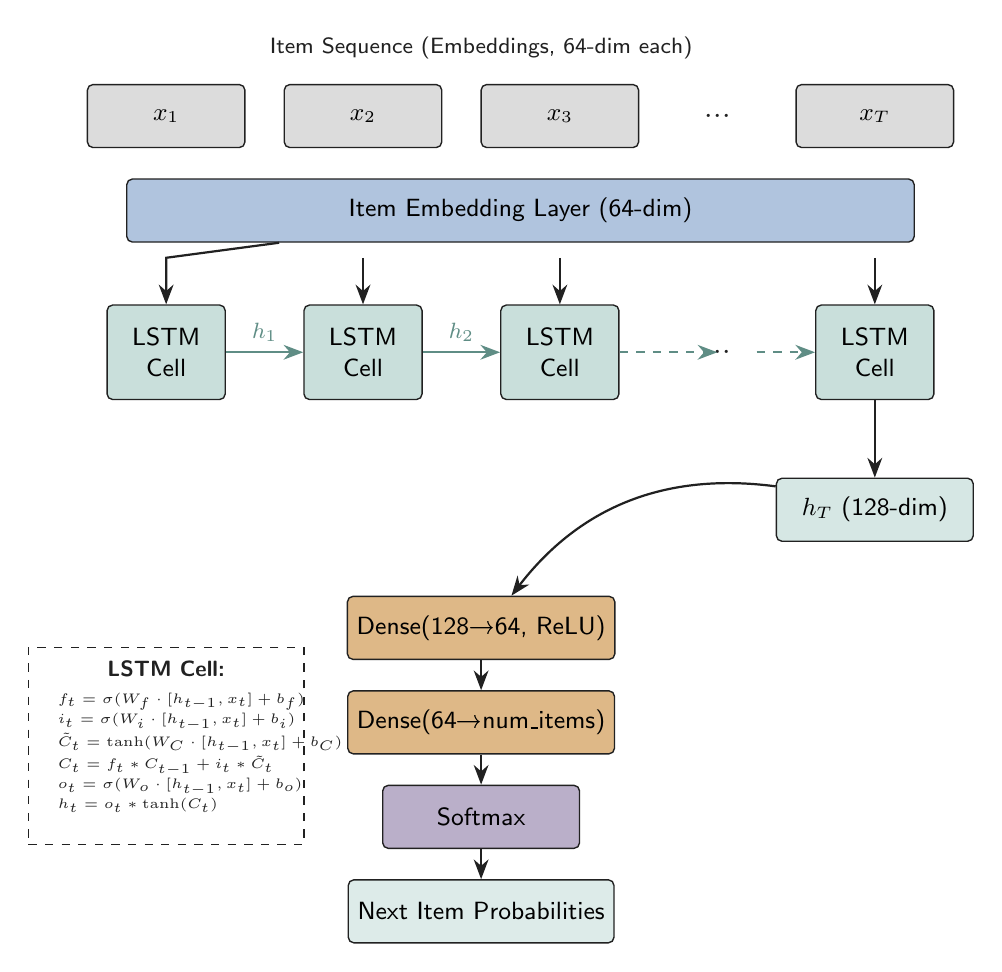
\begin{tikzpicture}[
    node distance=1cm,
    layer/.style={rectangle, draw=textdark, rounded corners=2pt, minimum width=2cm, minimum height=0.8cm, align=center, font=\small\sffamily, line width=0.5pt},
    lstm/.style={rectangle, draw=textdark, rounded corners=2pt, fill=lstmteal!40, minimum width=1.5cm, minimum height=1.2cm, align=center, font=\small\sffamily, line width=0.5pt},
    arrow/.style={-{Stealth[length=2.5mm]}, thick, color=textdark},
]

% Input sequence
\node[layer, fill=inputgray] (x1) at (-4, 5) {$x_1$};
\node[layer, fill=inputgray] (x2) at (-1.5, 5) {$x_2$};
\node[layer, fill=inputgray] (x3) at (1, 5) {$x_3$};
\node[font=\large, color=textdark] at (3, 5) {...};
\node[layer, fill=inputgray] (xn) at (5, 5) {$x_T$};

\node[font=\footnotesize\sffamily, anchor=south, color=textdark] at (0, 5.6) {Item Sequence (Embeddings, 64-dim each)};

% Embedding layer
\node[layer, fill=embedblue, minimum width=10cm] (embed) at (0.5, 3.8) {Item Embedding Layer (64-dim)};

% LSTM cells
\node[lstm] (lstm1) at (-4, 2) {LSTM\\Cell};
\node[lstm] (lstm2) at (-1.5, 2) {LSTM\\Cell};
\node[lstm] (lstm3) at (1, 2) {LSTM\\Cell};
\node[font=\large, color=textdark] at (3, 2) {...};
\node[lstm] (lstmn) at (5, 2) {LSTM\\Cell};

% Hidden states
\draw[arrow, color=lstmteal!80!black] (lstm1) -- node[above, font=\footnotesize\sffamily] {$h_1$} (lstm2);
\draw[arrow, color=lstmteal!80!black] (lstm2) -- node[above, font=\footnotesize\sffamily] {$h_2$} (lstm3);
\draw[arrow, dashed, color=lstmteal!80!black] (lstm3) -- (3, 2);
\draw[arrow, dashed, color=lstmteal!80!black] (3.5, 2) -- (lstmn);

% Connections from embedding to LSTM
\draw[arrow] (embed) -- (-4, 3.2) -- (lstm1);
\draw[arrow] (-1.5, 3.2) -- (lstm2);
\draw[arrow] (1, 3.2) -- (lstm3);
\draw[arrow] (5, 3.2) -- (lstmn);

% Final hidden state
\node[layer, fill=lstmteal!30, minimum width=2.5cm] (hfinal) at (5, 0) {$h_T$ (128-dim)};
\draw[arrow] (lstmn) -- (hfinal);

% Dense layers
\node[layer, fill=denseorange, minimum width=3cm] (dense1) at (0, -1.5) {Dense(128→64, ReLU)};
\node[layer, fill=denseorange, minimum width=3cm] (dense2) at (0, -2.7) {Dense(64→num\_items)};
\node[layer, fill=outputpurple, minimum width=2.5cm] (softmax) at (0, -3.9) {Softmax};
\node[layer, fill=lstmteal!25] (out) at (0, -5.1) {Next Item Probabilities};

\draw[arrow] (hfinal) to[bend right=30] (dense1);
\draw[arrow] (dense1) -- (dense2);
\draw[arrow] (dense2) -- (softmax);
\draw[arrow] (softmax) -- (out);

% LSTM cell detail (small box)
\node[rectangle, draw=textdark, dashed, minimum width=3.5cm, minimum height=2.5cm, line width=0.5pt] (detail) at (-4, -3) {};
\node[font=\footnotesize\bfseries\sffamily, anchor=north, color=textdark] at (-4, -1.8) {LSTM Cell:};
\node[font=\tiny\sffamily, align=left, anchor=north west, color=textdark] at (-5.5, -2.2) {
$f_t = \sigma(W_f \cdot [h_{t-1}, x_t] + b_f)$\\
$i_t = \sigma(W_i \cdot [h_{t-1}, x_t] + b_i)$\\
$\tilde{C}_t = \tanh(W_C \cdot [h_{t-1}, x_t] + b_C)$\\
$C_t = f_t * C_{t-1} + i_t * \tilde{C}_t$\\
$o_t = \sigma(W_o \cdot [h_{t-1}, x_t] + b_o)$\\
$h_t = o_t * \tanh(C_t)$
};

\end{tikzpicture}
\end{document}
